% ============================================================
\chapter{Convex Sets}
\label{ch:convex_sets}
% ============================================================

Imagine stretching a rubber band between two pins stuck in a piece of
cardboard. The band follows a straight line. Now imagine that the accessible
region of the cardboard is constrained: if, no matter where you place the
two pins \emph{within} the region, the rubber band stays entirely inside it,
then that region is \emph{convex}. This is an idea as old as geometry itself
--- Euclid knew about convex polygons --- but its consequences for
optimization are profound and were only fully exploited in the twentieth
century, by pioneers like Minkowski, Fenchel, Rockafellar, and Boyd.

% ------------------------------------------------------------
\section{Introduction and Motivation}
% ------------------------------------------------------------

Convex sets are the fundamental building blocks of convex optimization. An optimization
problem is called convex when one minimizes a convex function over a convex set. The
geometry of these sets determines the structure of solutions and guides algorithm design.

\begin{intuition}
A set is convex if, for every pair of points in the set, the line segment connecting
them lies entirely within the set. This simple property has profound consequences:
every local minimum is global, and hyperplane separation techniques become available.
\end{intuition}

\section{Fundamental Definitions}

\begin{definition}[Convex Set]
A set $C \subseteq \R^n$ is \emph{convex} if, for all $x, y \in C$ and all
$\theta \in [0,1]$:
\[
    \theta x + (1-\theta)y \in C.
\]
\end{definition}

\begin{definition}[Convex Combination]
A point $x$ is a \emph{convex combination} of points $x_1, \ldots, x_k$ if there
exist $\theta_1, \ldots, \theta_k \geq 0$ with $\sum_{i=1}^k \theta_i = 1$ such that:
\[
    x = \sum_{i=1}^k \theta_i x_i.
\]
\end{definition}

\begin{definition}[Convex Hull]
The \emph{convex hull} of a set $S \subseteq \R^n$, denoted $\mathrm{conv}(S)$,
is the set of all convex combinations of points in $S$:
\[
    \mathrm{conv}(S) = \left\{ \sum_{i=1}^k \theta_i x_i \;\middle|\;
    x_i \in S, \; \theta_i \geq 0, \; \sum_{i=1}^k \theta_i = 1, \; k \in \N^* \right\}.
\]
\end{definition}

\begin{theorem}[Carath\'eodory]
\label{thm:caratheodory}
Let $S \subseteq \R^n$. Every point in $\mathrm{conv}(S)$ can be written as a convex
combination of at most $n+1$ points in $S$.
\end{theorem}

\begin{proof}
Let $x \in \mathrm{conv}(S)$. Then $x = \sum_{i=1}^k \theta_i x_i$ with
$\theta_i > 0$, $\sum \theta_i = 1$, $x_i \in S$. If $k > n+1$, the vectors
$x_2 - x_1, \ldots, x_k - x_1$ number $k-1 > n$ and are therefore linearly
dependent. There exist $\mu_2, \ldots, \mu_k$, not all zero, such that
$\sum_{i=2}^k \mu_i (x_i - x_1) = 0$. Set $\mu_1 = -\sum_{i=2}^k \mu_i$.
Then $\sum_{i=1}^k \mu_i x_i = 0$ and $\sum_{i=1}^k \mu_i = 0$.

For $t \in \R$, $x = \sum_{i=1}^k (\theta_i - t\mu_i)x_i$. Choose
$t^* = \min_{i:\mu_i>0} \theta_i/\mu_i$. Then $\theta_i - t^*\mu_i \geq 0$
for all $i$, and at least one coefficient vanishes, reducing the number of terms.
Iterate until $k \leq n+1$.
\end{proof}

\section{Examples of Convex Sets}

\begin{example}[Classical Convex Sets]
The following sets are convex:
\begin{enumerate}
    \item \textbf{Hyperplane}: $\{x \in \R^n \mid \inner{a}{x} = b\}$ with $a \neq 0$.
    \item \textbf{Halfspace}: $\{x \in \R^n \mid \inner{a}{x} \leq b\}$.
    \item \textbf{Euclidean ball}: $B(x_0, r) = \{x \mid \norm{x - x_0} \leq r\}$.
    \item \textbf{Ellipsoid}: $\{x \mid (x-x_0)^T P^{-1}(x-x_0) \leq 1\}$, $P \succ 0$.
    \item \textbf{Polyhedron}: $\{x \mid Ax \leq b, \; Cx = d\}$.
    \item \textbf{Simplex}: $\Delta_n = \{x \in \R^n_+ \mid \sum x_i = 1\}$.
    \item \textbf{PSD cone}: $\mathbb{S}^n_+ = \{X \in \mathbb{S}^n \mid X \succeq 0\}$.
\end{enumerate}
\end{example}

\begin{proof}[Verification for the ball]
Let $x, y \in B(x_0, r)$ and $\theta \in [0,1]$. By the triangle inequality:
\[
    \norm{\theta x + (1-\theta)y - x_0}
    = \norm{\theta(x-x_0) + (1-\theta)(y-x_0)}
    \leq \theta\norm{x-x_0} + (1-\theta)\norm{y-x_0}
    \leq \theta r + (1-\theta)r = r.
\]
\end{proof}

\section{Convex Cones}

\begin{definition}[Cone]
A set $K \subseteq \R^n$ is a \emph{cone} if for all $x \in K$ and all
$\lambda \geq 0$, we have $\lambda x \in K$.
\end{definition}

\begin{definition}[Convex Cone]
A cone $K$ is \emph{convex} if $K$ is a convex set, which is equivalent to:
for all $x, y \in K$ and $\lambda, \mu \geq 0$:
\[
    \lambda x + \mu y \in K.
\]
\end{definition}

\begin{definition}[Dual Cone]
The \emph{dual cone} of $K$ is:
\[
    K^* = \{y \in \R^n \mid \inner{y}{x} \geq 0, \; \forall x \in K\}.
\]
\end{definition}

\begin{proposition}[Properties of the Dual Cone]
\label{prop:dual_cone}
\begin{enumerate}
    \item $K^*$ is a closed convex cone.
    \item If $K_1 \subseteq K_2$, then $K_2^* \subseteq K_1^*$.
    \item If $K$ is a closed convex cone, then $K^{**} = K$.
\end{enumerate}
\end{proposition}

\begin{example}[Classical Dual Cones]
\begin{itemize}
    \item The dual cone of $\R^n_+$ is $\R^n_+$ (self-dual).
    \item The dual cone of the Lorentz cone
    $\mathcal{L}^n = \{(x,t) \in \R^{n-1} \times \R \mid \norm{x} \leq t\}$
    is $\mathcal{L}^n$ itself.
    \item The dual cone of $\mathbb{S}^n_+$ is $\mathbb{S}^n_+$.
\end{itemize}
\end{example}

\section{Operations Preserving Convexity}

\begin{theorem}[Convexity-Preserving Operations]
\label{thm:operations}
The following operations preserve convexity:
\begin{enumerate}
    \item \textbf{Intersection}: if $C_\alpha$ is convex for all $\alpha \in I$,
          then $\bigcap_{\alpha \in I} C_\alpha$ is convex.
    \item \textbf{Affine image}: if $C$ is convex and $f(x) = Ax + b$, then
          $f(C) = \{Ax + b \mid x \in C\}$ is convex.
    \item \textbf{Affine preimage}: if $C$ is convex, then
          $f^{-1}(C) = \{x \mid Ax + b \in C\}$ is convex.
    \item \textbf{Minkowski sum}: if $C_1, C_2$ are convex, then
          $C_1 + C_2 = \{x + y \mid x \in C_1, y \in C_2\}$ is convex.
    \item \textbf{Projection}: if $C \subseteq \R^n \times \R^m$ is convex, then
          $\{x \in \R^n \mid \exists y, (x,y) \in C\}$ is convex.
    \item \textbf{Perspective function}: if $C$ is convex and $P(x,t) = x/t$ for
          $t > 0$, then $P(C)$ is convex.
\end{enumerate}
\end{theorem}

\begin{proof}[Proof of (1)]
Let $x, y \in \bigcap_\alpha C_\alpha$ and $\theta \in [0,1]$. For each $\alpha$,
$x, y \in C_\alpha$, so $\theta x + (1-\theta)y \in C_\alpha$ by convexity of
$C_\alpha$. Thus $\theta x + (1-\theta)y \in \bigcap_\alpha C_\alpha$.
\end{proof}

\begin{remark}
The union of two convex sets is generally not convex. For example, $\{0\} \cup \{1\}$
is not convex in $\R$. Arbitrary intersection preserves convexity, but union does not.
\end{remark}

\section{Separation Theorems}

\begin{theorem}[Hyperplane Separation]
\label{thm:separation}
Let $C, D \subseteq \R^n$ be two nonempty disjoint convex sets. There exists
$a \in \R^n$, $a \neq 0$, and $b \in \R$ such that:
\[
    \inner{a}{x} \leq b \; \forall x \in C
    \quad \text{and} \quad
    \inner{a}{x} \geq b \; \forall x \in D.
\]
\end{theorem}

\begin{theorem}[Strict Separation]
\label{thm:strict_separation}
Let $C$ be a nonempty closed convex set and $x_0 \notin C$. There exists
$a \in \R^n$, $a \neq 0$, and $b \in \R$ such that:
\[
    \inner{a}{x_0} > b > \inner{a}{x} \quad \forall x \in C.
\]
\end{theorem}

\begin{proof}
Let $\bar{x} = \mathrm{proj}_C(x_0)$ be the projection of $x_0$ onto $C$ (which
exists and is unique since $C$ is closed and convex). Set $a = x_0 - \bar{x}$ and
$b = \inner{a}{\bar{x}} + \frac{1}{2}\norm{a}^2$.

For all $x \in C$, the projection characterization gives:
\[
    \inner{x_0 - \bar{x}}{x - \bar{x}} \leq 0,
\]
that is, $\inner{a}{x} \leq \inner{a}{\bar{x}}$. Moreover:
\[
    \inner{a}{x_0} = \inner{a}{\bar{x}} + \norm{a}^2 > \inner{a}{\bar{x}} + \tfrac{1}{2}\norm{a}^2 = b > \inner{a}{\bar{x}} \geq \inner{a}{x}.
\]
\end{proof}

\begin{intuition}
Geometrically, the separation theorem states that one can always place a hyperplane
between two disjoint convex sets. This is the higher-dimensional analogue of the fact
that two disjoint intervals on the real line can be separated by a point.
\end{intuition}

\section{Supporting Hyperplanes}

\begin{definition}[Supporting Hyperplane]
Let $C \subseteq \R^n$ be a convex set. A \emph{supporting hyperplane} of $C$ at a
boundary point $x_0 \in \partial C$ is a hyperplane $H = \{x \mid \inner{a}{x} = b\}$
such that:
\[
    \inner{a}{x_0} = b \quad \text{and} \quad
    \inner{a}{x} \leq b \; \forall x \in C.
\]
\end{definition}

\begin{theorem}[Existence of Supporting Hyperplanes]
Let $C$ be a nonempty convex set with nonempty interior, and $x_0 \in \partial C$.
Then there exists a supporting hyperplane of $C$ at $x_0$.
\end{theorem}

\section{Support Function and Indicator Function}

\begin{definition}[Support Function]
The \emph{support function} of a set $C$ is:
\[
    \sigma_C(y) = \sup_{x \in C} \inner{y}{x}.
\]
\end{definition}

\begin{definition}[Convex Indicator Function]
The \emph{indicator function} (in the sense of convex analysis) of $C$ is:
\[
    \iota_C(x) = \begin{cases} 0 & \text{if } x \in C, \\ +\infty & \text{otherwise.} \end{cases}
\]
\end{definition}

\begin{proposition}
If $C$ is a nonempty closed convex set, then $\iota_C$ is convex, proper, and lower
semicontinuous. Moreover, $\sigma_C = \iota_C^*$ (the Fenchel conjugate of $\iota_C$).
\end{proposition}

\section{Projection onto a Closed Convex Set}

\begin{theorem}[Convex Projection]
\label{thm:projection}
Let $C \subseteq \R^n$ be a nonempty closed convex set. For every $y \in \R^n$,
there exists a unique $\bar{x} \in C$ such that:
\[
    \bar{x} = \argmin_{x \in C} \norm{x - y}^2.
\]
This point, denoted $\mathrm{proj}_C(y)$, is characterized by:
\[
    \bar{x} \in C \quad \text{and} \quad
    \inner{y - \bar{x}}{x - \bar{x}} \leq 0, \quad \forall x \in C.
\]
\end{theorem}

\begin{proof}
\textbf{Existence.} Let $d = \inf_{x \in C} \norm{x - y}$. Take $(x_k) \subset C$
with $\norm{x_k - y} \to d$. By the parallelogram identity:
\[
    \norm{x_k - x_l}^2 = 2\norm{x_k - y}^2 + 2\norm{x_l - y}^2 - 4\norm{\tfrac{x_k+x_l}{2} - y}^2.
\]
Since $\frac{x_k+x_l}{2} \in C$ (convexity), $\norm{\frac{x_k+x_l}{2} - y} \geq d$, so:
\[
    \norm{x_k - x_l}^2 \leq 2\norm{x_k - y}^2 + 2\norm{x_l - y}^2 - 4d^2 \to 0.
\]
$(x_k)$ is Cauchy, hence converges to $\bar{x} \in C$ (since $C$ is closed).

\textbf{Uniqueness.} If $\bar{x}_1, \bar{x}_2$ are two projections, the same argument
shows $\norm{\bar{x}_1 - \bar{x}_2} = 0$.

\textbf{Characterization.} $\bar{x}$ minimizes $\varphi(x) = \norm{x-y}^2$ over $C$
if and only if for all $x \in C$ and $t \in (0,1]$:
$\varphi(\bar{x} + t(x-\bar{x})) \geq \varphi(\bar{x})$, which gives
$\inner{y - \bar{x}}{x - \bar{x}} \leq 0$.
\end{proof}

\begin{proposition}[Non-expansiveness of Projection]
The projection $\mathrm{proj}_C$ is non-expansive:
\[
    \norm{\mathrm{proj}_C(x) - \mathrm{proj}_C(y)} \leq \norm{x - y}, \quad \forall x, y \in \R^n.
\]
In particular, $\mathrm{proj}_C$ is continuous (Lipschitz with constant $1$).
\end{proposition}

\section{Polyhedra and Representations}

\begin{definition}[Polyhedron]
A \emph{polyhedron} is the intersection of finitely many halfspaces:
\[
    P = \{x \in \R^n \mid Ax \leq b\}, \quad A \in \R^{m \times n}, \; b \in \R^m.
\]
A bounded polyhedron is called a \emph{polytope}.
\end{definition}

\begin{theorem}[Minkowski--Weyl]
A set $P \subseteq \R^n$ is a polytope if and only if it is the convex hull of
finitely many points:
\[
    P = \mathrm{conv}(\{v_1, \ldots, v_k\}).
\]
More generally, every polyhedron admits a representation of the form:
\[
    P = \mathrm{conv}(\{v_1, \ldots, v_k\}) + \mathrm{cone}(\{d_1, \ldots, d_l\}).
\]
\end{theorem}

\section{Geometric Interpretation}

\begin{center}
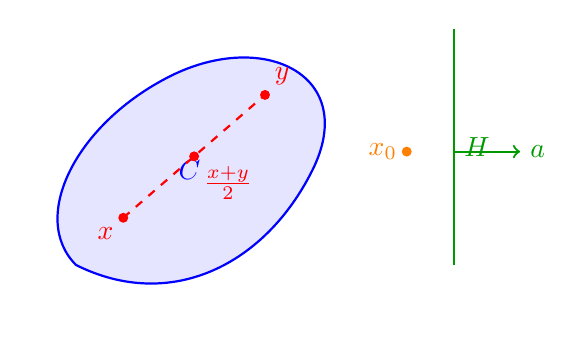
\begin{tikzpicture}[scale=1.2]
    % Convex set
    \draw[thick, blue, fill=blue!10]
        (0,0) .. controls (1,-0.5) and (2,0) ..
        (2.5,1) .. controls (3,2) and (2,2.5) ..
        (1,2) .. controls (0,1.5) and (-0.5,0.5) .. (0,0);
    \node[blue] at (1.2,1) {$C$};

    % Two points and segment
    \fill[red] (0.5,0.5) circle (1.5pt) node[below left] {$x$};
    \fill[red] (2,1.8) circle (1.5pt) node[above right] {$y$};
    \draw[red, thick, dashed] (0.5,0.5) -- (2,1.8);

    % Midpoint
    \fill[red] (1.25,1.15) circle (1.5pt) node[below right]
        {$\frac{x+y}{2}$};

    % Separating hyperplane
    \draw[thick, green!60!black] (4,0) -- (4,2.5)
        node[midway, right] {$H$};
    \fill[orange] (3.5,1.2) circle (1.5pt) node[left] {$x_0$};
    \draw[->, thick, green!60!black] (4,1.2) -- (4.7,1.2) node[right] {$a$};
\end{tikzpicture}
\end{center}

\section{Python Implementation}

\begin{codeblock}[title=\textbf{Simplex projection and convexity verification}]
\begin{minted}{python}
import numpy as np
import matplotlib.pyplot as plt

def project_simplex(v):
    """Project onto the standard simplex."""
    n = len(v)
    u = np.sort(v)[::-1]
    cumsum = np.cumsum(u)
    rho = np.max(np.where(u + (1 - cumsum) / (np.arange(n) + 1) > 0))
    theta = (cumsum[rho] - 1) / (rho + 1)
    return np.maximum(v - theta, 0)

def is_convex_hull_member(point, vertices):
    """Check if point is in conv(vertices) via LP."""
    import scipy.optimize as opt
    k = len(vertices)
    V = np.array(vertices).T  # n x k
    n = V.shape[0]
    c = np.zeros(k)
    A_eq = np.vstack([V, np.ones((1, k))])
    b_eq = np.append(point, 1.0)
    bounds = [(0, None)] * k
    res = opt.linprog(c, A_eq=A_eq, b_eq=b_eq, bounds=bounds)
    return res.success

# Demonstration: simplex projection
np.random.seed(42)
v = np.random.randn(3)
p = project_simplex(v)
print(f"Original point: {v}")
print(f"Projection:     {p}")
print(f"Sum = {p.sum():.6f}, min = {p.min():.6f}")
\end{minted}
\end{codeblock}

\section{Exercises}

\begin{exercise}[$\star$]
Show that the intersection of two halfspaces is convex.
\end{exercise}

\begin{exercise}[$\star$]
Show that the image of a convex set under a linear map is convex.
\end{exercise}

\begin{exercise}[$\star\star$]
Let $C = \{x \in \R^n \mid \norm{x}_1 \leq 1\}$. Show that $C$ is a polytope
and determine its vertices.
\end{exercise}

\begin{exercise}[$\star\star$]
Let $C$ be a closed convex set and $x_0 \notin C$. Prove that there exists a unique
closest point $\bar{x} \in C$ to $x_0$. Show that
$\inner{x_0 - \bar{x}}{x - \bar{x}} \leq 0$ for all $x \in C$.
\end{exercise}

\begin{exercise}[$\star\star$]
Compute the dual cone of the Lorentz cone
$\mathcal{L}^n = \{(x,t) \in \R^{n-1}\times\R \mid \norm{x} \leq t\}$.
\end{exercise}

\begin{exercise}[$\star\star\star$]
Prove Carath\'eodory's theorem geometrically in dimension 2, then generalize
the proof to dimension $n$.
\end{exercise}

\begin{exercise}[$\star\star\star$]
Let $f : \R^n \to \R$ be continuous. Show that the sublevel set
$\{x \mid f(x) \leq \alpha\}$ is closed. Give an example showing it is not
necessarily convex even if $f$ is continuous.
\end{exercise}
